
\documentclass[draft,linenumbers]{agujournal}
\draftfalse
\journalname{Journal of Advances in Modeling Earth Systems (JAMES)}
\begin{document}


\title{Implementing plant hydraulics in the Community Land Model}
\authors{Daniel Kennedy\affil{1},
Sean Swenson\affil{2},
Keith Oleson\affil{2},
David Lawrence\affil{2},
Rosie Fisher\affil{2},
Pierre Gentine\affil{1}
}


\affiliation{1}{Columbia}
\affiliation{2}{NCAR}
\correspondingauthor{Daniel Kennedy}{djk2120@columbia.edu}

\begin{keypoints}
\item = enter point 1 here = 
\item = enter point 2 here = 
\item = enter point 3 here = 
\end{keypoints}


\begin{abstract}
= enter abstract here xx =
\end{abstract}

%====================
%  INTRODUCTION
%====================

\section{Introduction}

 - droughts are increasing 
      . \citep{cook2015}
      . \citep{dai2013}
      . amazon dry season lengthening \citep{fu2013}

 - vapor pressure deficit 
      . \citep{mcdowell2015}
      . \citep{novick2016b}
      . \citep{williams2013}

 - with lingering uncertainty in veg response
      . \citep{dekauwe2017}
      . \citep{friedlingstein2014}
      . \citep{anderegg2015b}


SPAC representation is important, defines:
  - vegetation water status
  - atmospheric carbon sink
  - hydrologic transpiration sink
  - magnitude and timing of transpiration

Representation in CLM is known deficiency
  - also in other models
      . \citep{powell2013,ukkola2016}


Adds complexity, is it worth it, tractable?
       . hydraulic traits too hard \citep{drake2017}?, but people are doing it \citep{xu2016,christoffersen2016}

  - Trait information is available \citep{kattge2011,anderegg2015a} and valuable \citep{choat2012}
  - Water status information available \citep{konings2016,grant2016} and valuable \citep{momen2017,konings2017b}
  - Model structural information
  
Our goal:
  - parsimonious plant hydraulic implementation
  - setting a framework to represent vegetation water status
       . opening an interface to trait data, satellite VOD \citep{momen2017}
       . improving functionality

%====================
%  MODEL DESCRIPTION
%====================
\section{Model Description}

%Photosynthesis
\subsection{Photosynthesis}
\label{sect:A}
    The CLM5 photosynthesis model is largely inherited from CLM4.5 as described in \citet{bonan2011}, \citet{thornton2007},
    and \citet{oleson2013}.Photosynthesis is defined in three regimes: Rubisco-limited, light-limited, and export-limited 
    following \citet{farquhar1980} and \citet{harley1992}.The implementation extends \citet{sellers1996a,sellers1996b} with 
    colimitation following \citet{collatz1991}. 
    
    CLM5 photosynthesis is a two-big-leaf model, with a sunlit and shaded leaf per PFT per gridcell \citep{thornton2007, 
    dai2004, oleson2013}. The canopy fluxes module iterates for leaf surface energy balance.
    Within this, the photosynthesis module iterates to solve for intercellular CO$_2$ concentration, balancing stomatal flux of 
    CO2 with photosynthetic assimilation flux of CO2.
    
    Vegetation water stress is implemented via the vegetation water stress factor ($f_w$, dimensionless, 0 to 1, formerly 
    $\beta_t$). This factor multiplies the rate of maximum carboxylation ($V_{\text{cmax}}$) as described in \citet{oleson2013} and first implemented in \citet{sellers1996a,sellers1996b}. 
    
    With PHS, $f_w$ replaces the CLM4.5 transpiration beta function ($\beta_t$). 
    These factors are used by the photosynthesis model in the same way, but calculated differently. 
    The parameterization for $f_w$ is based on leaf water potential (see Section \ref{sect:demand}) . 
    For $\beta_t$, the parameterization is based on soil water potential (see Section \ref{sect:btran}).
    The switch to leaf water potential adopts the framework where stomatal conductance optimized for carbon gain is concurrently limited by hydraulic constraints \citep{novick2016a}


%Stomatal Conductance
\subsection{Stomatal Conductance}
\label{sect:gs}
    CLM5 uses the Medlyn stomatal conductance model, which reconciles the empirical and optimal approaches to modeling 
    stomatal conductance \citep{medlyn2011}. 
    Stomatal conductance of CO2 is related to net photosynthesis ($A_n$), atmospheric CO2 concentration at the leaf surface 
    ($C_a$), and the square root of the vapor pressure deficit near the leaf surface ($\sqrt{D}$).
    \begin{equation}
    g_s=g_0+\left(1+\dfrac{g_1}{\sqrt{D}}\right)\dfrac{A}{C_a}
    \end{equation}
    The model features two parameters $g_0$ ($\mu$mol / m2 / s) and $g_1$ (kPa$^{0.5}$). The $g_0$ parameter fits a 
    minimum stomatal conductance. The $g_1$ parameter relates to the water cost guiding the optimization of carbon 
    assimilation.
    
    The attenuation of stomatal conductance due to water stress follows the CLM4.5 formulation as described in 
    \citet{oleson2013} and \citet{bonan2011}. Prognostic water stress ($f_w$, ranging from 0-1) attenuates stomatal 
    conductance indirectly via multiplication of $V_{\text{cmax}}$. 

% Plant Hydaulics
\subsection{Plant Hydraulic Stress (PHS)}
  We implemented a simplified plant hydraulic framework in CLM. 
  Using hydraulic laws and the corresponding circuit analogy, we represent the 
  flow of water through the soil-plant-atmosphere continuum. 
  The hydraulic framework is used to effect water stress associated with increasing xylem tension
  and for calculating the soil transpiration sink for each soil layer. 
  Water stress attenuation of transpiration and photosynthesis is based on prognostic leaf water potential. 
  Design decisions followed a preference for a simplified implementation that,
  whenever possible, conformed to existing CLM architecture.
  We refer to the combined water supply and demand implementations as Plant Hydraulic Stress (PHS).
  
  \begin{figure}[h]
     \centering
     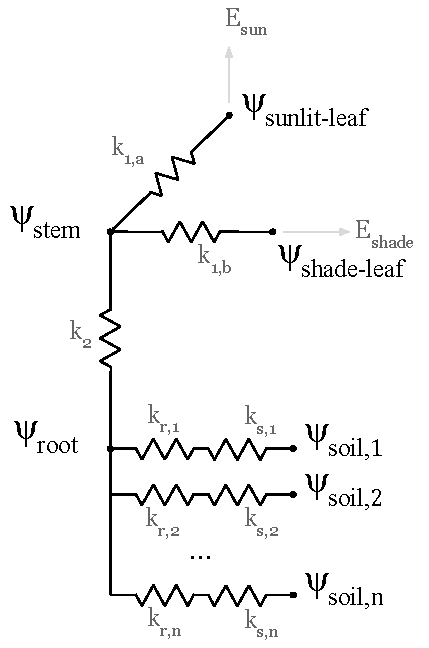
\includegraphics[width=9pc]{../figs/circuit.pdf}
     \caption{Plant hydraulic circuit analog schematic}
     \label{circuit}
  \end{figure}

%Hydraulic schematic and segmentation
  \subsubsection{Hydraulic schematic and segmentation}
  PHS solves for the set of vegetation water potential values 
  ($\psi_{\text{root}}$, $\psi_{\text{stem}}$, $\psi_{\text{shade-leaf}}$, $\psi_{\text{sun-leaf}}$ ) 
  that matches water supply (root water uptake) to water demand (transpiration), 
  while maintaining continuity of water flow throughout the soil-plant-atmosphere continuum.
  The PHS circuit analogy is presented in Figure \ref{circuit}.
  At each node, we resolve water potential, and, between nodes, we resolve the flux of water.
  The resistors define the segment conductance to water. 
  The segmentation is designed to take advantage of field-measured hydraulic traits 
  and to conform to the existing CLM architecture.
  From CLM, we inherit the vertically discretized soil layers and the two-layer (sunlit vs. shaded) canopy.
  From the hydraulic theory, we additionally segment the resistance across the soil matrix from the 
  resistance through root tissue \citep{williams1996}. 
  Likewise we segment the resistances through the root, stem, and leaf tissue to allow for differences
  in their parameterizations \citep{simonin2015, sperry2015}.

%Water Supply
    \subsubsection{Water supply}
    \label{sect:supply}
    Water supply is modeled via Darcy's Law where flow is proportional to the gradient in water potential. 
    Flow of water ($q$) is the product of the path hydraulic conductance ($k$) and 
    the gradient in water potential (accounting for change in gravitational potential). 
    Equation \ref{eq:darcy} represents the flow from node 1 to node 2. 
    
     \begin{linenomath*}
     \begin{equation}
     \label{eq:darcy}
     q = k\left(\psi_1 - \psi_2 - \rho g \Delta z\right)
     \end{equation}
     \end{linenomath*}
    
    PHS does not represent plant tissue water storage (by circuit analogy: capacitance). 
    Capacitance significantly complicates the water potential solution \citep{celia1990}
    and is challenging to parameterize \citep{bartlett2016}.
    However, buffering of water stress provided by tissue water storage can be important
    especially on sub-daily timescales \citep{meinzer2009}, whereby its inclusion may be warranted 
    in future model generations.

     Vegetation segment conductance is modeled with empirical xylem vulnerability curves \citep{tyree1989}, 
     where segments lose conductance with increasing drought status associated with 
     cavitation and embolism \citep{holbrook2001}.
     The vulnerability curves model loss of conductance relative to maximum conductance using two parameters: 
     $c_k$, a sigmoidal shape-fitting parameter, and 
     $p_{50}$, the water potential at 50\% loss of segment conductance (following \cite{gentine2016}). 
     These parameters can be estimated from field experiments \citep{sack2002}, 
     and $p_{50}$ is available in the TRY trait database \citep{kattge2011}.
     Parameterization based on $p_{50}$ is especially attractive in light of the call for transition to
     a trait-based model paradigm \citep{anderegg2015a}.
     The loss of xylem conductivity is based on lower terminus water potential ($\psi_1$)
     as is typical in other simplified models \citep{xu2016}, but 
     may underestimate the integrated loss of conductivity \citep{sperry2015}. 
         
     \begin{linenomath*}
     \begin{equation}
     \label{eq:vulnerability}
     k = k_{\text{max}} \, 2^{-\left(\dfrac{\psi_1}{p_{50}}\right)^{c_k}}
     \end{equation}
     \end{linenomath*}
     
     PHS models root, stem, and leaf conductances according to equation \ref{eq:vulnerability}.
     The parameterization of $k_{\text{max}}$ varies by hydraulic segment (see details in Appendix zqz).
     The conductance across the matrix from soil to root follows \citet{williams2001} and \citet{bonan2014} 
     to estimate the distance between roots for the length-scaling of soil conductance.
     Bulk soil resistivity is based on \citet{clapp1978} as described in \citet{oleson2013}.
     For a more complete description see Appendix zqz.
    
%Water demand
    \subsubsection{Water demand}
    \label{sect:demand}
    
    Water demand is based on the Medlyn stomatal conductance model (see Section \ref{sect:gs}), 
    which we adjust for water stress with $f_w$, the PHS water stress factor. 
    The water stress factor attenuates stomatal conductance indirectly, multiplying $V_{\text{cmax}}$.
    We calculate the water stress factor based on leaf water potential, such that 
    as leaf water potentials decrease, stress increases.
    The PHS stress factor is different from the CLM4.5 stress function, because that one 
    is calculated based on soil potential.
    The PHS stress factor is the same as the CLM4.5 stress function in that, once calculated, they are used
    to attenuate photosynthesis and stomatal conductance in the same way.

    
     \begin{linenomath*}
     \begin{eqnarray}
     \begin{aligned}
     \label{eq:demand}
     E_{\text{sun}}     &= E_{\text{sun,max}} \, 2^{-\left(\dfrac{\psi_{\text{sun-leaf}}}{\psi_{50}}\right)^{c_k}} \\
     E_{\text{shade}} &= E_{\text{shade,max}} \, 2^{-\left(\dfrac{\psi_{\text{shade-leaf}}}{\psi_{50}}\right)^{c_k}}
     \end{aligned}
     \end{eqnarray}
     \end{linenomath*}
    
    
     \begin{linenomath*}
     \begin{eqnarray}
     \begin{aligned}
     \label{eq:stress}
     f_{\text{w,sun}}         &= \dfrac{g_{\text{s,sun}}}{g_{\text{s,sun,max}}} \\
     f_{\text{w,shade}}     &= \dfrac{g_{\text{s,shade}}}{g_{\text{s,shade,max}}} \\
     \end{aligned}
     \end{eqnarray}
     \end{linenomath*}
    
    We define $f_w$ as the ratio of stressed to unstressed stomatal conductance (Equation \ref{eq:stress}).
    The unstressed stomatal conductance is the stomatal conductance when calculated with $f_w=1$
    (i.e. without water stress). 
    The "stressed" stomatal conductance is the stomatal conductance associated with the PHS module
    water flow solution, which matches vegetation water supply with vegetation water demand 
    (Section \ref{sect:solution}).
    This solution is the set of vegetation water potentials ($\psi$) where water supply
    (a generally increasing function of $\left|\psi\right|$) matches water demand
    (a generally decreasing function of $\left|\psi\right|$).
    The decrease of water demand at lower potentials is modeled with a two-parameter sigmoidal function 
     applied to maximum transpiration (Equation \ref{eq:demand}). 
     The parameters are $\psi_{50}$, the leaf water potential at 50\% loss of transpiration and 
     $c_k$ a sigmoidal shape-fitting parameter.
     
     Whereas the water supply parameters (see Section \ref{sect:supply}) 
     relate to hydraulic traits often measured in the field, 
     the hydraulic demand parameters $\psi_{50}$ and $c_k$ reflect the emergent property of stomatal control
     and must be empirically derived. 
     Likewise CLM4.5 had two empirical stomatal control parameters, which were the soil matric potentials 
     corresponding to stomates fully closed and stomates fully open (see Section \ref{sect:btran}).
     The functional form of stomatal control is not generally agreed upon, and as such, 
     should be investigated farther. Recent modeling studies suggest sperry,xu,christo.

%PHS solution
    \subsubsection{PHS solution}
    \label{sect:solution}
    
    PHS solves for the set of vegetation water potential values ($\psi$) that matches water supply
    (root water uptake) to water demand (transpiration), while satisfying continuity across the four water flow
    segments (soil-to-root, root-to-stem, stem-to-leaf, and leaf-to-transpiration). 
    We compute the flux divergence $f$ (representing the mismatch of flow in and out of each segment)
    for a given set of vegetation water potential values $\psi_i$, and iteratively update $\psi$ until $f\to0$.
    
    \begin{linenomath*}
    \begin{equation} 
    \psi = \left[
    \begin{array}{c}
    \psi_{\text{sun}} \\ 
    \psi_{\text{shade}} \\ 
    \psi_{\text{stem}} \\ 
    \psi_{\text{root}}            
    \end{array} \right]
    \end{equation}
    \end{linenomath*}
    
    \begin{linenomath*}
    \begin{equation}
    f\left(\psi\right) = \left[ 
    \begin{array}{c}
    E_{sun}-q_{sun}\\
    E_{shade}-q_{shade}\\
    q_{sun}+q_{shade}-q_{stem}\\
    q_{stem}-\sum_{j=1}^n{q_{root,j}}
    \end{array} \right]
    \end{equation}
    \end{linenomath*}
    
    \begin{linenomath*}
    \begin{equation}
    A = \dfrac{df}{d\psi}
    \end{equation}
    \end{linenomath*}    
    
    While $\left|f\right|>0$
    \begin{linenomath*}
    \begin{equation} \begin{aligned}
    \label{eq:iter}
    \Delta\psi &=A^{-1}f\left(\psi_i\right) \\
    \psi_{i+1}  &= \psi_i + \Delta\psi
    \end{aligned} \end{equation}
    \end{linenomath*}    
    
    The numerics are especially tractable because $f$ has analytical derivatives and $A$ 
    (a 4x4 matrix with six null entries) is easily inverted when well-conditioned. 
    Supply and demand converge, because transpiration demand decreases with more negative 
    leaf water potentials and supply increases with more negative leaf water potentials.
    
    Furthermore several simplifications were made that decreases the numerical complexity.
    For the purposes of the PHS solution, soil potentials are assumed constant during each timestep.
    During each PHS iteration (\ref{eq:iter}), transpiration is assumed to be linear with $f_w$,
    which precludes updating leaf temperature and intercellular CO$_2$.
    Plant tissue water storage (capacitance) is not represented, whereby the solution does not
    depend on the previous timestep and has no time derivatives.

%====================
%  EXP DESCRIPTION
%====================
\section{Experiment Description}
    
\section{Analysis Methods}    
    
%====================
%  BTRAN
%====================

\section{Water stress factor, SMS vs. PHS}
\label{sect:btran}
    PHS alters the transpiration beta function ($\beta_t$, colloquially BTRAN), 
    which is the phenomenological soil water stress function in CLM2-CLM4.5, as described in \citet{oleson2013}.
    Because the name $\beta_t$ is associated with this specific plant hydrodynamics representation, we opt to rename the variable to $f_w$ (water stress factor).
    Throughout this paper we refer to the CLM4.5 plant hydrodynamics framework as SMS (soil moisture stress), 
    as compared to the newer implementation, PHS (plant hydraulic stress).
    We adopt this terminology (in lieu of CLM4.5 vs. CLM5), because SMS is still deployable with CLM5. 
    All simulations in this paper use the same development version of CLM5, changing only the plant hydrodynamics model and the throughfall forcing.
    In this section we present the SMS version of $f_w$ and outline the differences as compared to PHS.
    
    With SMS, $f_w$ is calculated based on soil matric potential, as a root-fraction weighted average of a soil layer wilting factor (Equation \ref{bt:1}).
    This value multiplies $v_{\text{cmax}}$, effecting attenuation of photosynthesis and transpiration with drought.
    Recent studies suggest that the SMS parameterization introduces model bias in turbulent fluxes \citep{bonan2014}
    and contributes to unrealistic drought response of photosynthesis and stomatal conductance \citep{powell2013}.
    Furthermore, if $f_w$ represents a plant hydraulic safety mechanism, attenuating stomatal conductance to avoid
    dangerously low leaf water potentials, it makes sense to represent more of the hydraulic architecture (a la SPA or PHS)
    and assess hydraulic safety based on prognostic leaf water potential.
    
    With SMS, $f_w$ also sets the framework for vegetation soil water extraction. 
    Each timestep, $f_w$ is calculated and used to solve for photosynthesis and transpiration.
    The transpiration flux must then be distributed among the vertically discretized soil layers.
    In the SMS framework, the transpiration sink is partitioned by layer according to the layer wilting factor and root fraction.
    This framework leaves out several key physical attributes of soil water extraction, which are addressed in the PHS implementation.
    
    $f_w$ is unitless, ranging from 0 to 1, with 1 corresponding to no water stress, and 0 corresponding to fully water stressed. 
    It is calculated based on a root-fraction weighted average of soil layer wilting factor ($w_i$), which is a bounded linear 
    function of soil water potential ($\psi_i$) relative to PFT parameters defining the soil potential with stomates fully open ($
    \psi_{o}$) and fully closed ($\psi_{c}$). Note that root fraction ($r_i$) must sum to 1.
    
    \begin{linenomath*}
    \begin{equation} f_w = \sum_{i=1}^{n}{r_iw_i}
    \label{bt:1}
    \end{equation}
    \begin{equation} 
    \label{bt:2}
    w_i=0 \leq \dfrac{\psi_i-\psi_{c}}{\psi_{o}-\psi_{c}} \leq 1
    \end{equation}
    \end{linenomath*}
    
    SMS uses $f_w$ to attenuate photosynthesis and stomatal conductance with soil water stress. 
    It is also used for modeling vegetation water extraction from the soil column. 
    The total transpiration ($T$) is partitioned among the soil layers, based on the $f_w$ framework of soil water availability. 
    For each soil layer ($i$), the flux to transpiration ($q_i$) is calculated as the layer root fraction times the layer wilting factor, normalized by $f_w$. 
    This guarantees that the total soil water extraction equals the transpiration.
    \begin{linenomath*}
    \begin{equation}
    \label{bt:4}
    q_i = \dfrac{r_i w_i}{f_w}T
    \end{equation}
    \end{linenomath*}
    
    The PHS implementation adopts a hydraulic framework for root water uptake, where the flux from Soil Layer $i$ ($q_i$) is 
    the product of the hydraulic conductance ($k_i$) and the gradient in water potential ($\Delta\psi$) driving the flow.
    That gradient is the difference between the root water potential ($\psi_{\text{root}}$) and the soil water potential ($\psi_i$), less changes in gravitational potential.
    \begin{linenomath*}
    \begin{equation}
        \begin{aligned}
    q_i &= k_i \Delta\psi \\
    \Delta\psi &= \left(\psi_{i}-\psi_{\text{root}}-\Delta\psi_{\rho g,i} \right)
    \label{phs:sink}
    \end{aligned}
    \end{equation}
    \end{linenomath*}
    
    With some manipulation, we recast (\ref{bt:4}) into the hydraulic framework. We define $T_{\text{max}}$, such that: $T = 
    f_w T_{\text{max}}$ and use this expression to replace $T$ in (\ref{bt:4}).  Likewise we replace $w_i$ in (\ref{bt:4}) with the 
    formula from (\ref{bt:2}).
    
    \begin{linenomath*}
    \begin{equation} 
    q_i = \dfrac{T_{\text{max}}}{\psi_{o}-\psi_{c}} r_i \left(\psi_i-\psi_{c} \right)
    \end{equation}
    \end{linenomath*}
    
    This yields SMS analogs for the two terms of Equation \ref{phs:sink}.
    \begin{linenomath*}
    \begin{equation} \begin{aligned}
    k_i &= r_i \, \dfrac{T_{max}}{\psi_{o}-\psi_{c}} \\
    \Delta\psi &= \psi_i - \psi_{c} \\
    \mbox{constrained by:} \qquad
    \Delta\psi &=
    \begin{cases}
    0                          & \text{if } \psi_i<\psi_{c}  \\
    \psi_{o}-\psi_{c} & \text{if } \psi_i>\psi_{o}
    \label{kb}
    \end{cases}
    \end{aligned}\end{equation}
    \end{linenomath*}
    
    In Figure \ref{fig:cond}, we compare conductance values derived from the PHS and SMS implementations.
    With SMS, $k$ is not explicitly modeled, so instead we infer $k$, 
    by dividing $q_i$ by $\Delta\psi$ as defined in Equation \ref{kb}.
    Furthermore, we interpret the constraint that $\Delta\psi$ be greater than or equal to zero to mean 
    that conductance is zero in non-conforming cases. As such, we say $k=0$ when $\Delta\psi<\text{1 kPa}$.
    
    Issues with the SMS representation of the soil transpiration sink: 
    
    (1) Constant pulling potential \\
    Darcy's Law governs the flow of water through the soil-plant-atmosphere continuum, 
    with fluxes proportional to the gradient in water potential. 
    With SMS, that gradient is defined for each soil layer as 
    the difference between the soil water potential in that layer ($\psi_i$) 
    and a constant parameter, the soil water potential when stomata are fully closed ($\psi_{c}$).
    It serves as the vegetation ``pulling'' potential for calculating the soil transpiration sink.
    Using a constant is inconsistent with extensive evidence from the field of dynamic vegetation water potential.
    Likewise the values for $\psi_{c}$ are quite negative, (-2.5 MPa for broadleaf evergreen tropical). 
    
    (2) Conductance dynamics \\
    In lieu of dynamic vegetation water potential, intra-day SMS soil sink dynamics derive from a highly variable conductance.
    As inferred in Equation \ref{kb}, SMS conductance is modeled as a function of $T_{max}$, and three constant parameters.
    $T_{max}$ is highly dynamic, responding to the diurnal course in transpiration demand.
    This is inconsistent with general principles of porous media flow, where conductivity is a function of the hydraulic architecture and its wetted status.
    Likewise, this representation of conductance does not represent the characteristic phenomenon where vessels lose conductance with drying.
      
    (3) No dependence on absolute root biomass \\
    As is typical, the SMS conductance is scaled by layer using an area basis.
    In this case the relative root fraction is used.
    With PHS, an absolute measure of root biomass is used (see Appendix Equation \ref{eq:rai}).
    An absolute measure better conforms with the physics of porous media flow and better responds to varying carbon allocation strategies.
    For example, with SMS, if root mass double in every soil layer, the root access to water remains unchanged.

    (4) Lacks penalties for extraction from depth \\
    PHS implements two penalties for extracting water from deep in the soil column that are missing from SMS.
    The first is minor, but water extracted from depth must overcome gravity. 
    This amounts to about 0.01 MPa per meter in depth. 
    This is missing from SMS and included with PHS. 
    Likewise SMS ignores that hydraulic conductance is generally taken to scale with the inverse of conducting length.
    In PHS, this is featured both in the conductance within root vessels and 
    in the conductance governing the flux across the soil matrix to the root surface.
    
    (5) Constraints \\
    With SMS, the gradient in water potential is constrained between 0 and 
    the range of soil potential between parameters for stomata fully open and closed (Equation \ref{kb}). 
    The upper constraint caps the gradient in water potential when soil potential reaches the value for stomata fully open.
    There is no physical basis for why this would not continue to increase until saturation.
    The lower constraint caps the gradient in water potential at zero, disallowing negative gradients.
    However, reversed water fluxes, caused by negative gradients in water potential, have been observed in the field.
    Both constraints are eschewed with PHS.     
    
\section{Results and Discussion}
\subsection{Modeling vegetation water potential}

The new plant hydraulics module (PHS) introduces a representation of vegetation water potential to CLM.
Vegetation water potential is modeled at four locations within the plant: at the root, stem, shaded, and sunlit leaf levels.
Figure \ref{fig:vwp} shows the average diurnal cycle of vegetation water potential for the 2003 dry season at Caxiuana for two experiments:
the first with ambient throughfall, and the second with 60\% of throughfall excluded. 
Both panels show the characteristic drop in water potential around midday and the expected sequencing with 
the leaf water potentials more negative than the stem, which is more negative than the root water potential.

The sequencing is difficult to distinguish from the plot, where stem, sunlit, shaded nearly overlap for both experiments. 
In the ambient simulation (Fig \ref{fig:vwp}a), midday (1p.m.) water potentials are -1.98, -1.97, -1.96 MPa 
for sunlit leaf, shaded leaf, and stem, respectively.
With throughfall exclusion (Fig \ref{fig:vwp}b) midday (1p.m.) water potentials decrease to -2.77, -2.76, -2.75 MPa, respectively.
The small difference between leaf and stem water potentials results from minimal resistance to water flow across this segment. 

Throughfall exclusion (TFE) lowers midday sunlit leaf water potential by 0.79 MPa compared to the ambient simulation.
This drop in water potential can be partitioned among the segments of water flow from soil to leaf.
In the ambient simulation, predawn (5am) root water potential is -0.075 MPa. 
With TFE, it falls to -0.36 MPa, resulting in a drop in predawn root water potential of 0.28 MPa relative to the ambient simulation. 
The potential drop from predawn to midday root water potential increases by 1.06 MPa with TFE 
(from 0.058 MPa, ambient, to 1.12 MPA, TFE).
The drop from root to stem acts in the opposite direction, decreasing from 1.85 MPa in the ambient simulation
to 1.29 MPa with TFE, attenuating the drop in water potential by 0.55 MPa.

\cite{fisher2006}
predicted water potential values are in range, average dry season observation = -2.47 MPa, 
with no statistically significant difference between AMB and TFE.
For us, LWP drop due to TFE is -0.79MPa, which can be partitioned into -0.28 MPa predawn, -1.06 soil-to-root drop, +0.55 root-to-leaf drop.
Stem drop abates, smaller because though PLC increases, transpiration decreases to larger effect.
Consistent with findings in \cite{fisher2006} of 
1) isohydric behavior
and
2) that most of the resistance is above ground, but that the added resistance from drying is predominately below ground.

\cite{fisher2006} report dry season soil potential as -0.17 MPa in the ambient plot and -0.66 MPa in the TFE plot.
These are drier than predawn root water potential in our simulations.
Likewise the difference between TFE and AMB is more than 3x larger in the observations than in our simulations.
This indicates that our simulations underestimate the forcing from throughfall exclusion, likely due to an overestimation of the 
soil column's ability to buffer drying.

The current PHS parameterization of stem-to-leaf resistance is relatively naive compared to the literature \citep{franks2007}
and could be improved in future versions. 
This results in little difference between stem, shaded, and sunlit leaf water potentials.
Likewise the current PHS parameterization eschews vegetation capacitance. \citep{meinzer2004}
This leads to instantaneous equilibration of water potential with soil moisture and atmospheric forcing.
Finally, hydraulic conductance hysteresis is absent from the PHS vulnerability parameterization, 
whereby xylem segments fully regain conducting capacity upon re-wetting.
This limits the influence of drought legacy, which has been shown to be significant for forest mortality \citep{anderegg2013}.
Our objective was to simplify the plant hydraulic representation for this first implementation, 
allowing that it will be of interest to investigate more extended process representation in future versions.

\subsection{Stress factor, annual cycle}

The Medlyn stomatal conductance model optimizes carbon gain relative to water costs, but does not represent hydraulic constraints.
Representing the influence of drought in combination with the Medlyn model is an area of active research \citep{zhou2013,novick2016a}.
Dating back to \cite{sellers1996a}, CLM has used a water stress factor (unitless, 0-1, stressed-unstressed), to attenuate $v_{\text{cmax}}$ with declining water status. Decreases in $v_{\text{cmax}}$ result in decreases in photosynthesis, stomatal conductance, and transpiration, coupled via the stomatal conductance model and through the intercellular CO$_2$ concentration.

Previously (SMS) water stress was an empirical function of root-zone soil matric potential (see Section \ref{sect:btran}).
With PHS, the water stress factor is modeled as a function of leaf water potential.
Once calculated, the implementation of the stress factor are the same (in that they both multiply $v_{\text{cmax}}$).
But the dynamics of the two formulations are quite different, because with SMS the stress factor only responds to changes in soil potential,
whereas with PHS the stress factor also responds to transpiration demand.

Figure \ref{fig:mm} shows monthly mean values of the water stress factor, gross primary productivity, and transpiration
over the three-year simulation showing PHS versus SMS under both ambient and 60\% excluded throughfall conditions.
Careful interpretation is required for comparison, because straight time-averaging PHS stress function is not appropriate due to coincident diurnal cycles in $f_w$ and potential photosynthesis.
As such we plot the average midday $f_w$ (see zqz).


ambient

SMS no stress (fw>0.99), 24 out of 36 months
PHS more stress, follows leaf water potential (Figure \ref{fig:vwp}).

PHS mins generally in September (high FSDS, high VPD).
SMS mins generally in December (min root-average SMP).

Effect of TFE accumulates. 
PHS, adds 30\% and 47\% in Nov 2002 and Nov 2003
SMS, adds 60\% and 88\% in Oct 2002 and Sept 2003.

Difference in sensitivity to TFE due to root water uptake (Sections zqz)
PHS suppresses IAV of GPP
Neither gets TFE, but PHS looks nice compared to ambient sap flux.

Discussion

(1) Why can't we match TFE (PHS)?
        - isohydricity
        - draining soil column
        - too efficient extracting water from depth
(2) But we're very excited about the dynamics of the factor
        - soil moisture stress vs. xylem tension stress

\subsection{Stress factor, diurnal cycle}

PHS introduces a diurnal cycle to $f_w$, the CLM water stress factor (Fig \ref{fig4}a). 
This follows the diurnal cycle in leaf water potential (e.g. Fig \ref{fig:vwp}a,b).
The SMS version of $f_w$ has no diurnal cycle because it depends only on soil potential.
Leaf water potential declines with decreasing soil potential, but also with increasing transpiration demand.
Transpiration demand is a function of VPD, solar radiation (via photosynthesis), and other variables.

The effects of VPD and soil potential are shown in Figure \ref{fig:vpd}, where we plot a subset of $f_w$ data from the four simulations. 
To emphasize the relationship with VPD, we subset for a small window in downwelling solar radiation (between 400 and 425 W/m2).
Furthermore, for the TFE simulations (panels $c$ and $d$), we also subset for years 2002 and 2003, because TFE was not active during most of 2001.
Points are colored based on soil potential, splitting the data from each plot into terciles, blue points are wettest, red points driest, and yellow points intermediate.
For details see (zqz).
As expected the SMS version of $f_w$ has a clear dependence on soil potential, but no relationship with VPD (Fig \ref{fig:vpd}b,d). 
Drier soil potentials are associated with lower values of $f_w$, which corresponds to more stress.
With PHS, there is a clear dependence of $f_w$ on VPD, with higher VPD associated with more stress.
Under ambient throughfall conditions (Fig\ref{fig:vpd}a) the soil water has minimal influence.
In Figure \ref{fig:vpd}c, TFE yields drier soils, showing the combined dependence of $f_w$ on VPD and soil water.

What is the stress factor? An acknowledgment that optimizing $A-\lambda E$ is not the full story of vegetation water use.
For example, plants must also manage the risk of cavitation associated with increasing xylem tension.
No one answer is accepted within the field for how to apply water stress to photosynthesis and stomatal conductance.
Some groups abandon optimizing $A-\lambda E$ in favor of hydraulic costs \citep{sperry2017}.
Some groups are exploring soil water adjustments to lambda \citep{manzoni2013b}, but this may underestimate drought effects \citep{zhou2013}.
Other groups are combining Medlyn stomatal conductance, with so-called non-stomatal limitation, attenuating vcmax or mesophyl conductance
(which feeds back through photosynthesis to lower stomatal conductance). \citep{egea2011,novick2016a}
We opt for a simplified form of this last approach, but don't claim superiority, but rather that stress parameterizations are an important topic for continued research.

But having said that, we do really like our approach.
We are taking the point of view that Medlyn well-watered makes sense, but needs a water status factor.
We are not changing the Medlyn parameters with drying, though that may be justified.
Soil water is a viable option for measuring water status \citep{drake2017}, but doesn't capture the dual effects of supply and demand on xylem tension.
So we couple Medlyn to vcmax attenuated based on leaf water potential.

\subsection{Conductance}

PHS calculates vegetation water potential.
The prognostic vegetation water potential has two interfaces with the model.
As above, it is used to effect drought stress for the photosynthesis/stomatal conductance routines.
But we also use it to calculate root water uptake in the Darcy framework where $q=k\Delta\psi$.
More typically, a heuristic is used to partition the transpiration sink throughout the soil column (need ref).
CLM (with SMS) based this on root fraction and a soil wilting factor, which can be recast into the hydraulic framework (Section \ref{sect:btran}).
Looking at the conductance values associated with root water uptake serves to highlight the differences between paradigms.

Soil-to-root conductance ($k_{sr}$) is modeled in PHS and is used to model root water uptake (see zqz).
With SMS, $k_{sr}$ is not explicitly modeled, but it can be inferred, by dividing the root water uptake by the SMS extraction gradient (see Section \ref{sect:btran}).
In Figure \ref{fig:cond}, we plot the time-series of conductance values from Soil Layer 3 (spans from 6 to 12 centimeters below the surface) under ambient throughfall conditions during 2003.

Well-watered values are very different, two orders of magnitude. 
Dynamics also very different, PHS conductance is relatively steady through the wet season (Fig \ref{fig:cond}a).
Through the dry season, the conductance generally declines with short resurgence episodes associated with rain events.
SMS is highly dynamic with more variability relative to the mean (Fig \ref{fig:cond}b).
During FMA-2003, mean daily standard deviation of Layer 3 conductance is 4.6e-12 s$^{-1}$ with PHS
and 9.9e-12 s$^{-1}$ with SMS, whereby in an absolute sense SMS standard deviation is about twice as large.
The difference is larger in a relative sense, as that standard deviation is 0.08\% of the mean FMA conductance with PHS
and 62.9\% of the mean FMA conductance with SMS.

SMS inferred conductance is tethered to transpiration (see Section \ref{sect:btran}), causing the high variance.
Likewise, SMS features a clear diurnal cycle in the inferred Layer 3 conductance (Supp Fig \ref{supp:cond}). 
Instead PHS uses brooks-corey and root xylem vulnerability to calculate conductance, which better reflects our understanding of the physical process and the temporal dynamics.
As a result conductance is less variable, with the expected responses to drydown (loss of conductance) and re-wetting (increased conductance).
This is reinforced by the results in Figure 7. 
With 60\% throughfall exclusion (Fig7a, dotted line), PHS conductance decreases, whereas with SMS, the daily mean conductance increases (Fig7b).

The average SMS and PHS Layer 3 conductance for well-watered conditions (i.e. wet season, ambient throughfall) differ by about two orders of magnitude.
The SMS extraction gradient is measured relative to $\psi_c$ (a parameter defining soil potential with stomates fully closed), which equals -2.5MPa for BET.
The PHS extraction gradient is relative to root water potential which during 2003 (ambient throughfall) varies between -0.02 and -0.23 MPa.
Even as a leaf pull -2.5 MPa is too large during the wet season, but it really doesn't make sense to pull from the leaves, because the soil layers aren't in parallel to the leaves. 
Near surface $\psi$, before stem pressure drop is the more appropriate driving force, and it varies seasonally, way lower than -2.5 wet season.

With TFE, PHS Layer 3 conductance can approach the values seen in SMS. 
The average Layer 3 conductance with PHS for August 2003 (60\%TFE) is 4.75e-11 s$^{-1}$ as compared to 3.89e-11 s$^{-1}$ for SMS.
This is a result of the orders of magnitude response of PHS soil-to-root conductance to changes in soil potential, which is as expected with soil conductances.
Inferred SMS conductance has no clear relationship with soil potential (Supp Fig \ref{supp:cond2}). 
SMS root water uptake uses a heuristic to partition transpiration, but its dynamics end up a bit backwards. 
It's a workaround that's necessary when you aren't modeling the gradient in water potential between vegetation and soil. 
But now we are, which is a big benefit of modeling vegetation water potential.

\subsection{Extraction via hydraulic gradient}

Dry season water uptake Figure \ref{fig7} 
ambient, 
PHS more surface extraction (Fig \ref{fig7}a)
SMS a bit more extraction from beyond 2 meters, but quite a bit more between 0.5 and 2 meters.
PHS surface extraction (Fig \ref{fig7}b, black/solid) responds to precip (Fig \ref{fig7}d),
SMS does not.

tfe,
curves flip in Figure \ref{fig7}a, now PHS has about twice the extraction from beyond 2m.
note how surface extraction decreases substantially for PHS (Fig \ref{fig7}b),
but increases slightly for SMS.
PHS continues to respond to precip.
SMS now has a slight response to precip.

Wet season Figure \ref{fig8}
A lot more precip, steadier precip.

ambient,
PHS more surface extraction. net extraction zero beyond about 85 centimeters
SMS gets more than half its water from beyond about 1 meter

tfe,
PHS surface extraction increases, in service of downward HR.
note that HR is not going to depth, but rather to between 1 and 4.6 meters
there is extraction beyond 4.6 meters (albeit minimal, 1.6e-6 mm/s)
SMS surface extraction increases 3.33 to 4.75 cm
SMS deep extraction decreases 21.6 to 17.2 cm
deep roots \citep{nepstad1994}

HR has been observed in the field \citep{oliveira2005}, and has been highlighted as an important missing feature from CLM \citep{lee2005}.
This functionality is precluded with SMS, which sets root water uptake to zero if the gradient in water potential is negative. 
The PHS implementation allows hydraulic redistribution and is discussed in the next section.

The advantage of the SMS type of heuristic is that it sets up guardrails.
Hydraulic redistribution is precluded and extraction is capped.
However the consequent dynamics and drought response are not in agreement with expectations.
PHS offers improved model structure, with a more reasonable drought response.
PHS also offers a process connection between soil potential and leaf water potential.
This is attractive, because it exposes the vegetation water dynamics representation to new streams of observational data, 
namely in-situ leaf water potential and remotely-sensed vegetation optical depth.
However, scale mismatch, parallel assumptions and parameter uncertainty may add up to hydraulics no more realistic than the heuristic.
Likewise it's clear that we'll have more work to constrain the degrees of freedom in the PHS RWU vector.
While there are advantages to both, it seems there is a lot we can learn more from the PHS style of implementation.
Root water extraction is a critical component of vegetation hydrodynamics and merits continued research.
PHS makes inroads into a better representation of root water extraction.
I'm interested in seeing this parameterization studied further. 
It's probably also worth investigating alternative heuristic approaches that improve upon SMS.
Either way, we should also find new ways to constrain root water uptake with observations.


\subsection{Hydraulic redistribution}

Figure \ref{fig9} shows the total hydraulic redistribution by month for 2003.
The darker shading shows the portion of HR that occurs at night [6pm,6am). 
Note that only PHS is simulations are shown, because SMS disallows hydraulic redistribution.

2003HRamb is 41.3 cm (10.3 day, 31.0 night)
2003HRtfe is 37.0 cm (11.5 day, 25.5 night)

For reference,
2003 T/ET for these two sims were, amb 120/137, tfe 99/115 cm

The TFE simulation has less HR overall in 2003, but more HR during wet months, Feb-June.

Supp Figure \ref{supp:hr}
HR predominately downwards during wet season (FMA)
HR in both directions during dry season (SON)

Flows out of layer2 can be fast, and can run round the clock.

Difficult to say whether this is reasonable.



\subsection{Soil profile}

Cumulative ET, three years \\
    4.13,
    3.82,
    4.39,
    3.74,

For comparison, total ambient precip is 6.7 meters

SMSamb Nov-03 rootfr-weighted average smp is -0.42MPa
SMStfe Nov-03 rootfr-weighted average smp is -2.18MPa
PHSamb Nov-03 average predawn root water potential is -0.08MPa
PHStfe Nov-03 average predawn root water potential is -0.37MPa

Fisher2007 quotes dry amb smp based on predawn leaf = -0.17 +/- 0.10
dry tfe smp based on predawn leaf = -0.71 +/- 0.31

SMS-tfe has less ET, but achieves much more negative root-zone smp
PHS-tfe actually has an overall drier soil column 1.54m of water, compared to 1.61m of water for SMS
SMS is pulling way too hard
Likewise SMS hydrology is very sensitive to the parameter $\psi_c$. 
Scanning in time at a certain depth, you can see soil dry down to -2.5MPa and hang there, never falling to -3.
Noting of course that $\psi_c$=-2.5MPa.
PHS has more flexibility, with the dynamic root water potential, and so there is not the same tendency to dry out to a certain level.
Note how the minimum smp for PHS gets lower each dry season.

My feeling is that the value for $\psi_c$ is really just tuned to get the photosynthesis/transpiration in range, 
and the soil moisture dynamics, with scarce observational constraints, are allowed to miss.

PHS has a bit less ground evap 17.4/14.9 cm compared to 18.8/17.4 cm

final thoughts



    
\clearpage    

\section{Figures}
  \begin{figure}[h]
     \centering
     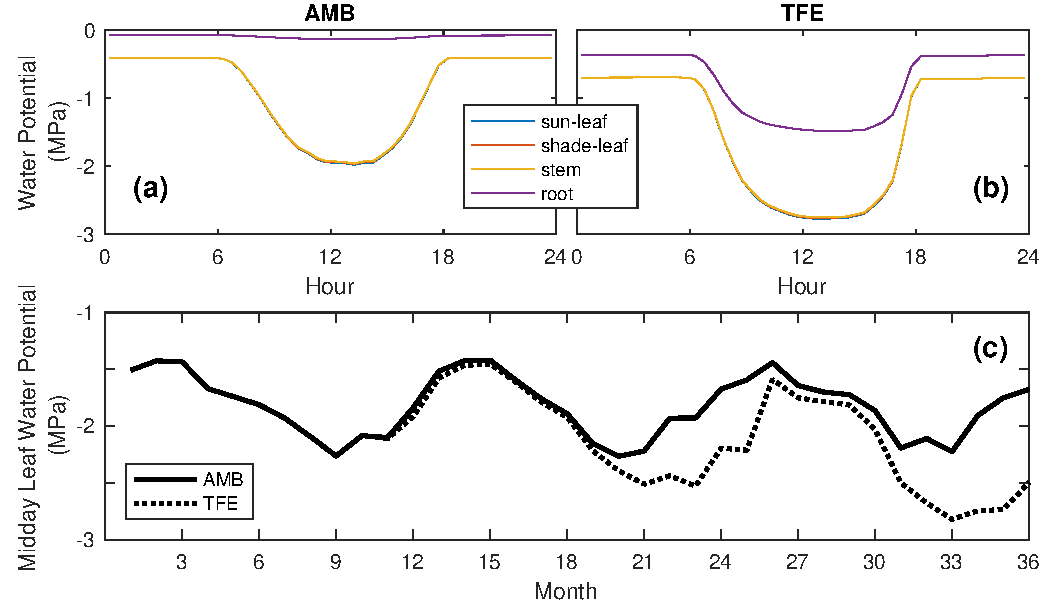
\includegraphics[width=30pc]{../figs2/fig2.pdf}
     \caption{Modeled vegetation water potential at  Caxiuan\~a, Brazil.
     (a) Dry season (SON) diurnal mean, ambient throughfall conditions,
     (b) Dry season (SON) diurnal mean, with 60\% throughfall excluded.
     Curves are drawn for sunlit leaf, shaded leaf, stem, and root water potentials. Note that the first three mostly overlap.
     (c) Monthly mean midday leaf water potential, under ambient (solid line) and 60\% throughfall exclusion (dotted line) conditions.
     Note that throughfall exclusion begins in month 11 (Nov 1, 2001).
     }
     \label{fig:vwp}
  \end{figure}
  
  \clearpage   
  \begin{figure}[h]
     \centering
     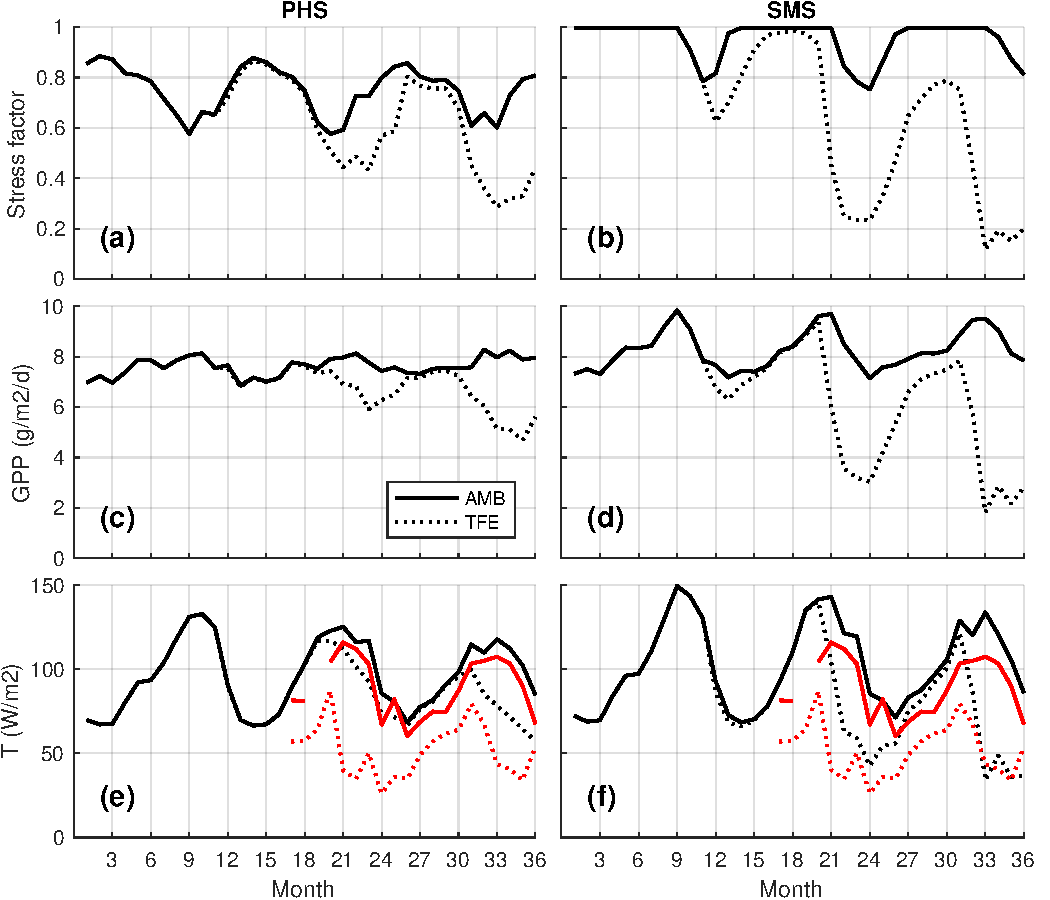
\includegraphics[width=30pc]{../figs2/fig3.pdf}
     \caption{(a,b) Monthly mean water stress function. Note that the water stress function equals 1 when there is no stress and 0 when fully stressed.
     (c,d) Monthly mean transpiration (W/m$^2$).
     (e,f) Monthly mean gross primary productivity (g/m$^2$/d). 
     Solid lines correspond to ambient throughfall conditions, and dotted lines feature 60\% throughfall exclusion.
     Black lines represent model output.
     Red lines show observational transpiration derived from sap flux (see zqz).
     PHS is on for (a), (c), and (e). PHS is off for (b), (d), and (f).
     }
     \label{fig:mm}
  \end{figure}
  
          \clearpage
    \begin{figure}[h]
     \centering
     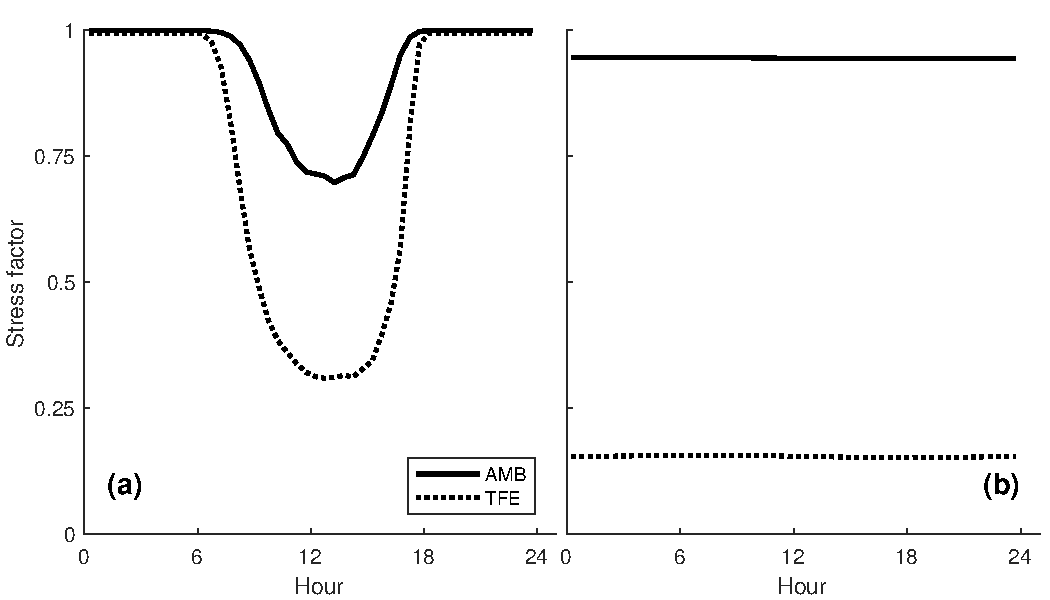
\includegraphics[width=30pc]{../figs2/fig4.pdf}
     \caption{2003 Dry season (SON) diurnal mean water stress function for 
     (a) PHS on, and
     (b) PHS off.
     Solid lines correspond to ambient throughfall conditions, and dotted lines feature 60\% throughfall exclusion.
     Note that the water stress function equals 1 when there is no stress and 0 when fully stressed.
     }
     \label{fig4}
  \end{figure}
  
      \clearpage
    \begin{figure}[h]
     \centering
     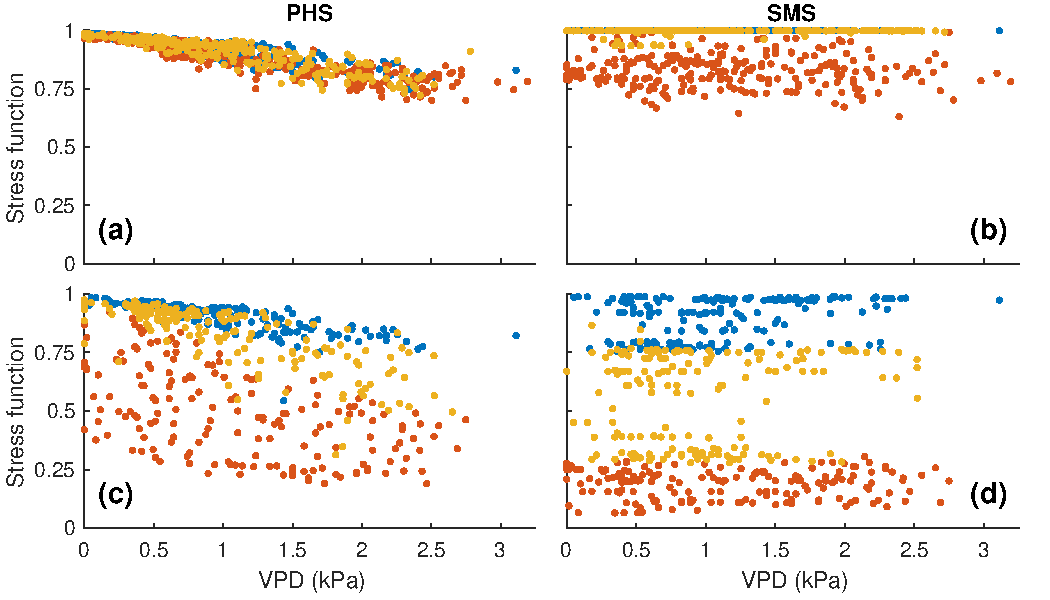
\includegraphics[width=30pc]{../figs2/fig5.pdf}
     \caption{Water stress function versus vapor pressure deficit, for points with downwelling shortwave radiation between 400 and 425 W/m2.
     (a) PHS, ambient throughfall
     (b) SMS, ambient throughfall
     (c) PHS, 60\% throughfall excluded
     (d) SMS, 60\% throughfall excluded. 
     For (a) and (c) data are subdivided based on predawn root water potential.
     For (b) and (d) data are subdivided based on average soil matric potential, weighted by root fraction.
     Blue dots represent the wettest tercile, yellow dots represent the intermediate tercile, and red dots represent the driest tercile.
     Note that panels (c) and (d) exclude data from 2001, when throughfall exclusion was not active.
     }
     \label{fig:vpd}
       \end{figure}
  
  
\clearpage   
  \begin{figure}[h]
     \centering
     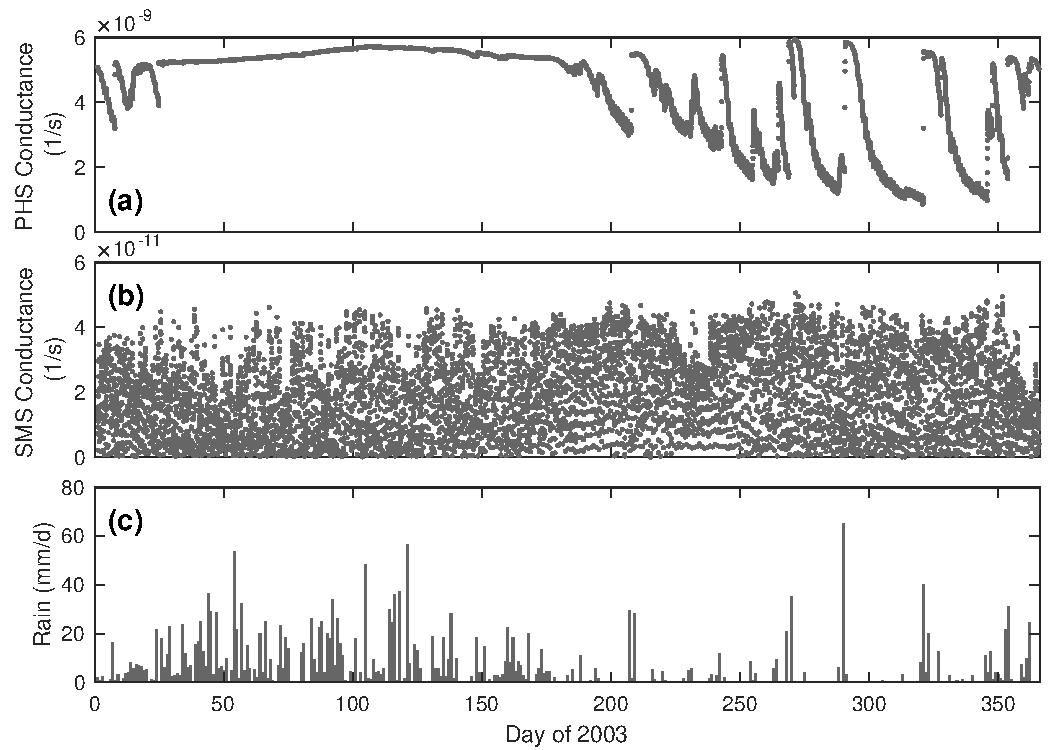
\includegraphics[width=30pc]{../figs2/fig6.pdf}
     \caption{Soil Layer 3 conductance, under ambient throughfall conditions in 2003. 
     (a) Time-series of PHS modeled soil-to-root conductance (s$^{-1}$) from Soil Layer 3 (spanning 6 to 12 centimeters in depth).
     (b) Time-series of SMS inferred conductance (s$^{-1}$) also from Soil Layer 3.
     (c) Concurrent precipitation forcing (mm/d).
     }
     \label{fig:cond}
  \end{figure}
  
  \clearpage   
  \begin{figure}[h]
     \centering
     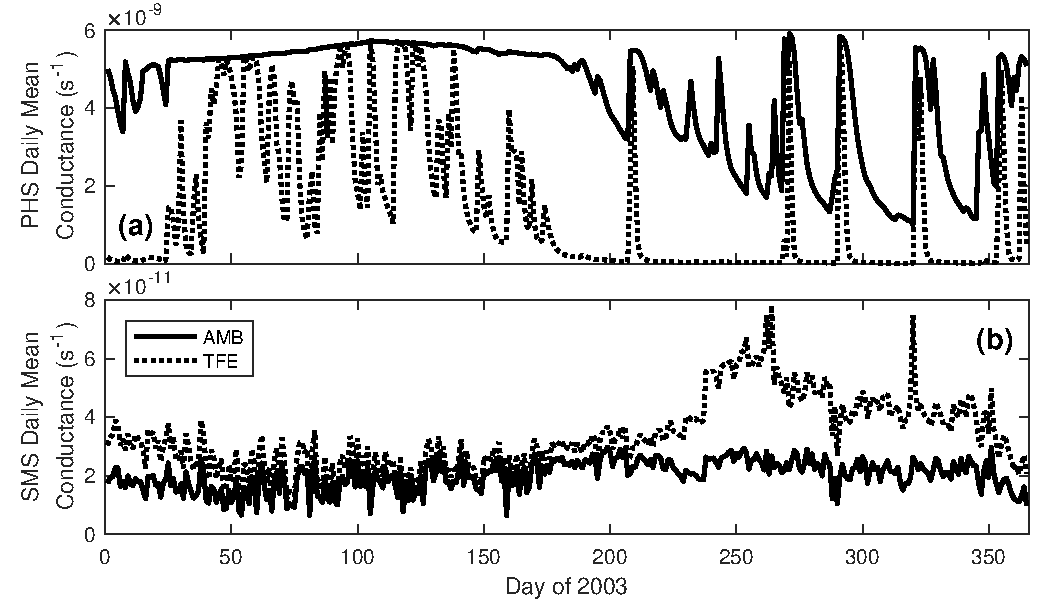
\includegraphics[width=30pc]{../figs2/fig6a.pdf}
     \caption{Daily mean Soil Layer 3 conductance, throughout 2003 under ambient (solid line) and 60\% throughfall exclusion (dotted line) conditions.
     (a) Daily mean of PHS modeled soil-to-root conductance (s$^{-1}$) from Soil Layer 3 (spanning 6 to 12 centimeters in depth).
     (b) Daily mean of SMS inferred conductance (s$^{-1}$) also from Soil Layer 3.
     }
     \label{fig:cond2}
  \end{figure}
  
        \clearpage
    \begin{figure}[h]
     \centering
     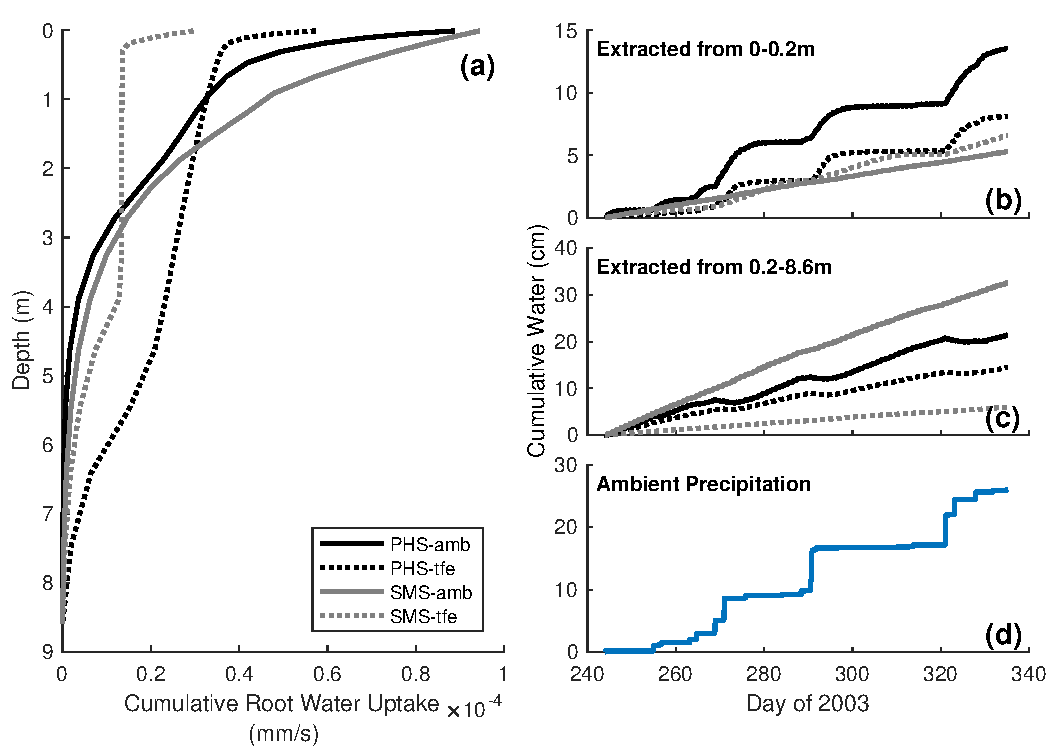
\includegraphics[width=30pc]{../figs2/fig7.pdf}
     \caption{2003 dry season (SON) root water uptake. 
     Panel (a) shows the average cumulative profile of daytime root water uptake (mm/s) for the four simulations during SON-2003.
     Panel (b) shows total water uptake from above 0.2m for the four simulations during SON-2003.
     Panel (c) shows total water uptake from below 0.2m for the four simulations during SON-2003. 
     Panel (d) shows total ambient precipitation during SON-2003. 
     }
     \label{fig7}
  \end{figure}
  
        \clearpage
    \begin{figure}[h]
     \centering
     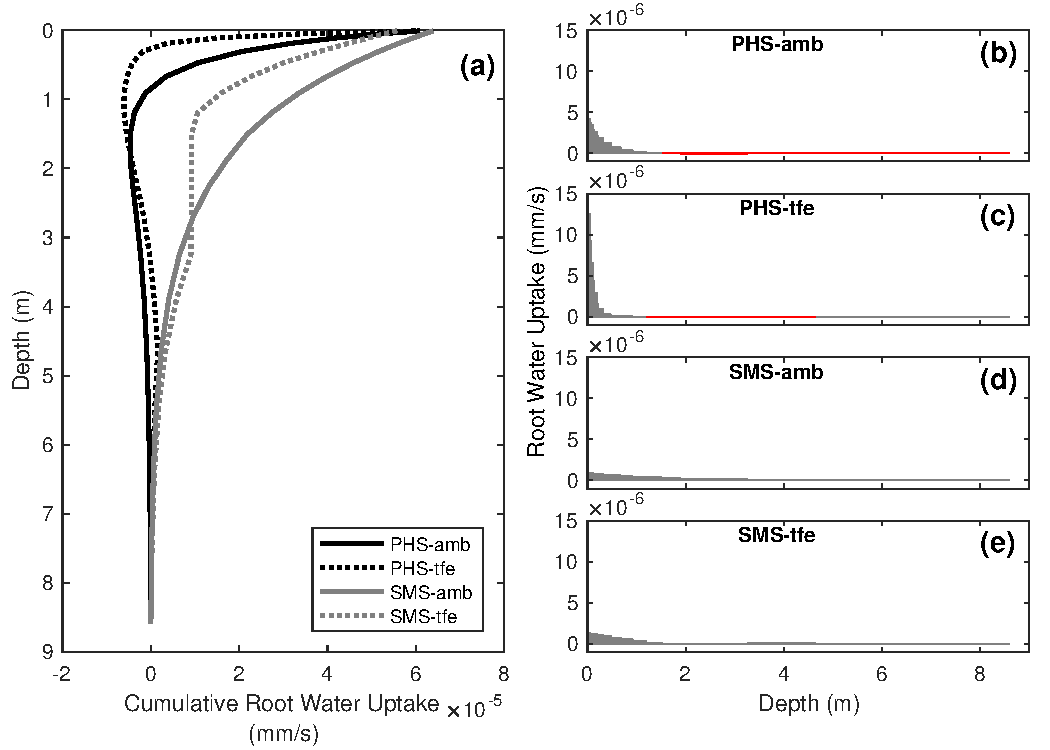
\includegraphics[width=30pc]{../figs2/fig8.pdf}
     \caption{2003 wet season (FMA) root water uptake. 
     Panel (a) shows the average cumulative profile of daytime root water uptake (mm/s) for the four simulations during FMA-2003.
     Panel (b) shows total water uptake from above 0.2m for the four simulations during FMA-2003.
     Panel (c) shows total water uptake from below 0.2m for the four simulations during FMA-2003. 
     Panel (d) shows total ambient precipitation during FMA-2003. 
     }
     \label{fig8}
  \end{figure}
  
    \clearpage
    \begin{figure}[h]
     \centering
     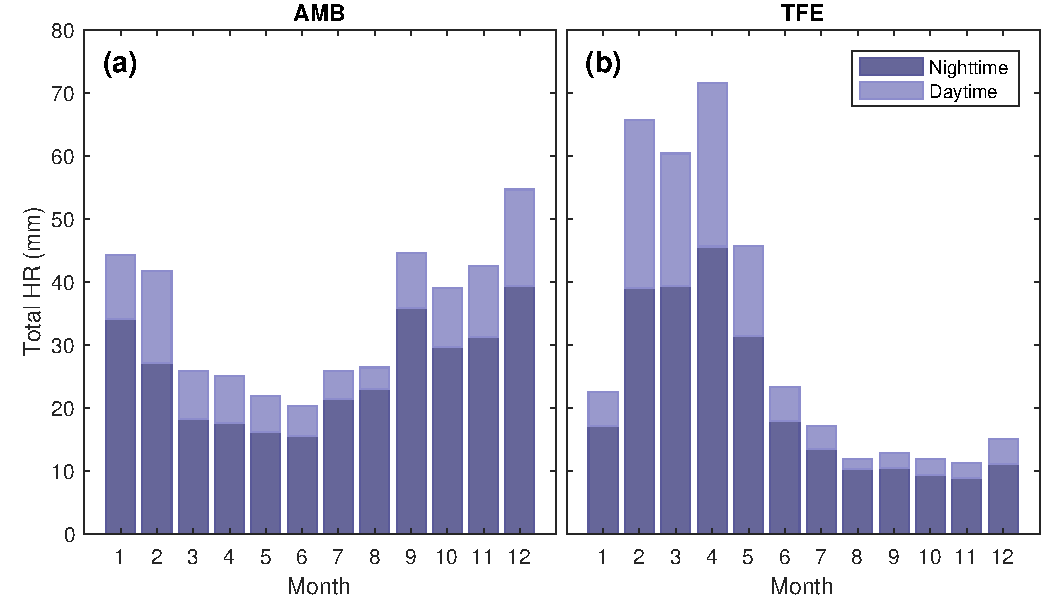
\includegraphics[width=30pc]{../figs2/fig9.pdf}
     \caption{Total hydraulic redistribution (mm) by month in 2003. For (a) ambient throughfall conditions, and (b) 60\% throughfall exclusion. 
     Darker shading shows portion of HR at night [6pm,6am), lighter shading shows portion of HR during day [6am,6pm).}
     \label{fig9}
  \end{figure}

  
      \clearpage
    \begin{figure}[h]
     \centering
     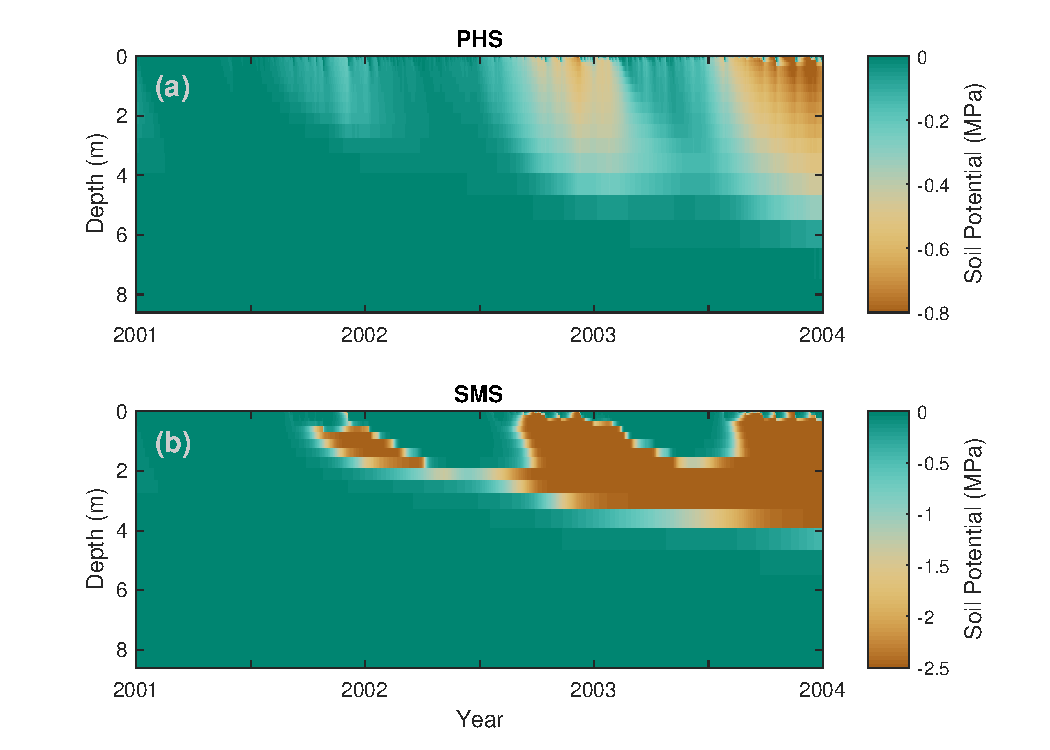
\includegraphics[width=30pc]{../figs2/fig11.pdf}
     \caption{Vertical profile of soil water potential (MPa) over time under 60\% throughfall exclusion, for
     (a) PHS, and 
     (b) SMS.
     Note that color axes are different. }
     \label{fig11}
  \end{figure}
  
  
  



  


\clearpage

\appendix
%====================
%  APPENDIX
%====================

\section{Supplementary Figures}

      \begin{figure}[h]
     \centering
     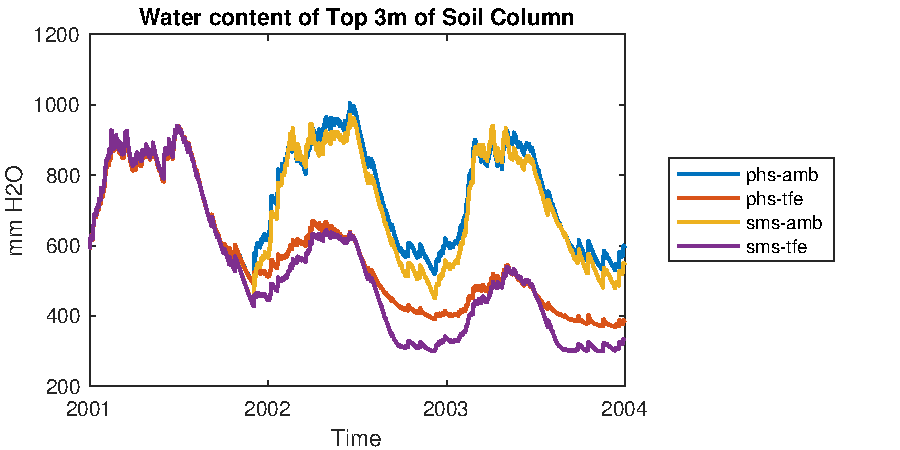
\includegraphics[width=30pc]{../figs2/top3m.pdf}
     \caption{Total water content of the top three meters of the soil column through time for the four simulations.}
     \label{top3m}
  \end{figure}
  \clearpage
  
        \begin{figure}[h]
     \centering
     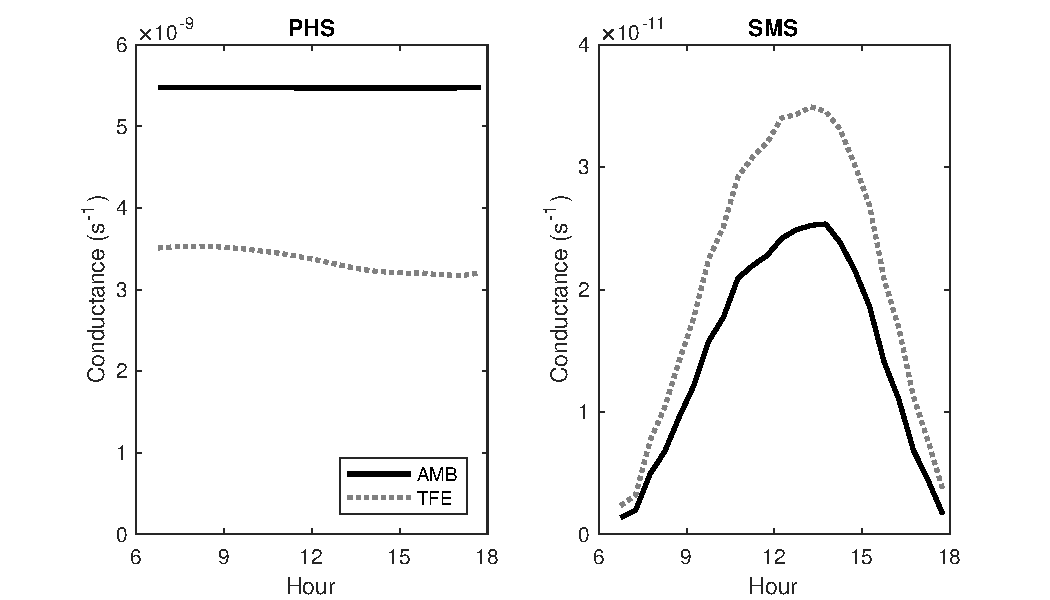
\includegraphics[width=30pc]{../figs2/suppfig1.pdf}
     \caption{FMA-2003 average diurnal cycle of layer 3 conductance.}
     \label{supp:cond}
  \end{figure}
  \clearpage
  
  \begin{figure}[h]
     \centering
     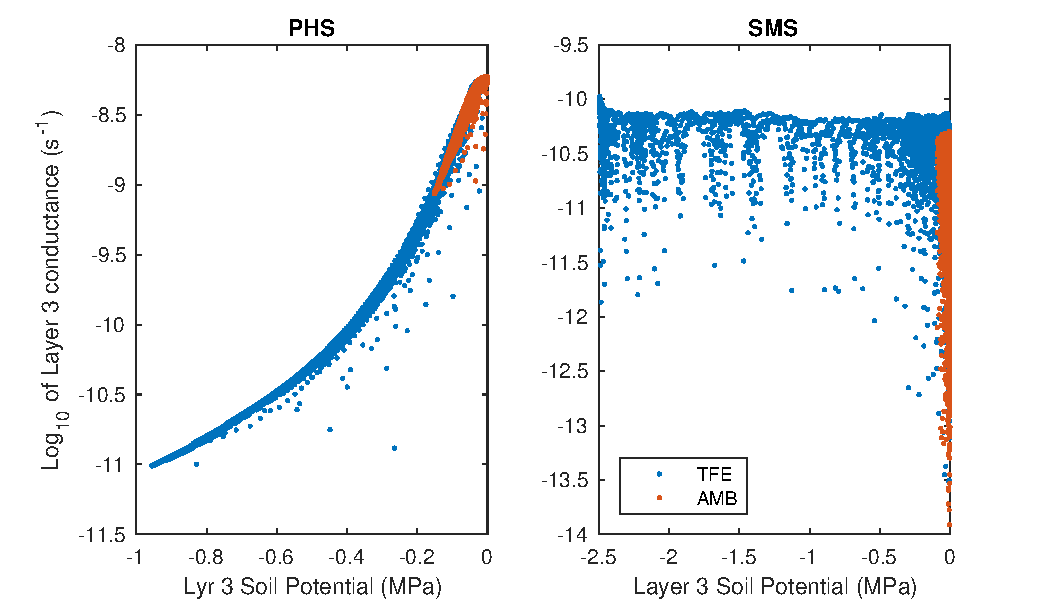
\includegraphics[width=30pc]{../figs2/suppfig2.pdf}
     \caption{Log of conductance versus soil potential for Soil Layer 3 (2003).}
     \label{supp:cond2}
  \end{figure}
  \clearpage

    \begin{figure}[h]
     \centering
     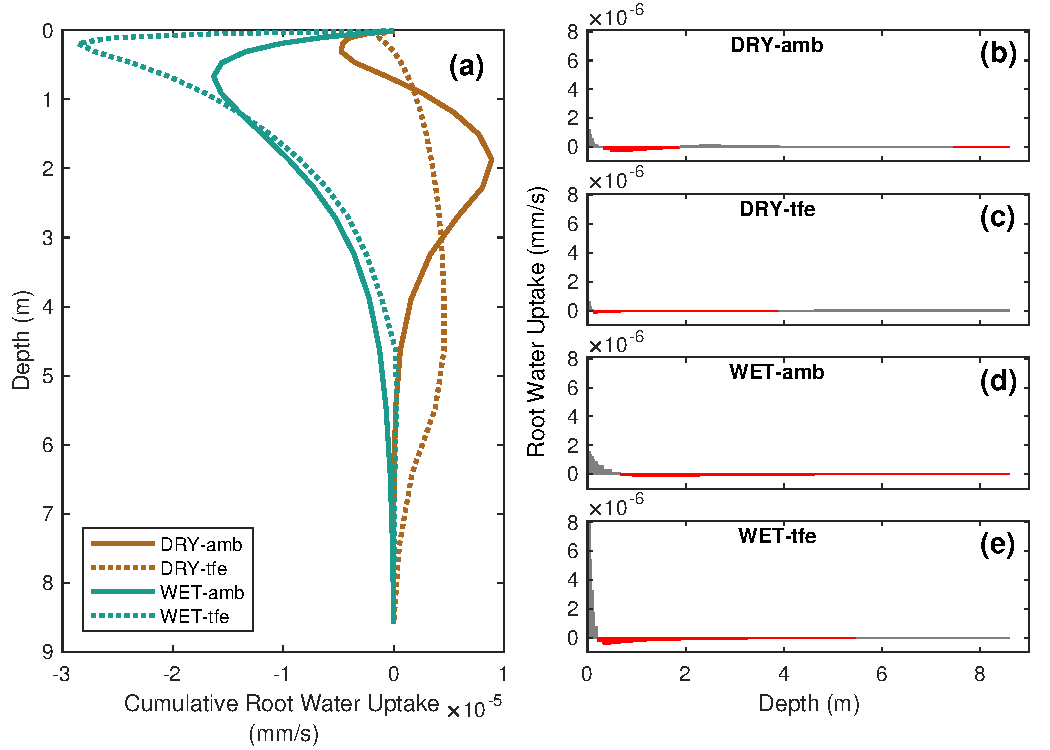
\includegraphics[width=30pc]{../figs2/fig10.pdf}
     \caption{PHS, nighttime (6pm to 6am) average root water uptake profiles with depth. 
     Panel (a) shows cumulative (starting at depth) root water uptake (mm/s) for ambient (solid line) and 60\% throughfall exclusion (dotted line)
     during the wet (FMA, cyan color) and dry (SON, brown color) seasons. 
     Panels (b)-(e) present the information from (a) in non-cumulative form. 
     Note that for panels (b)-(e) negative root water uptake is shaded red, and also that for panel (a), 
     when the positive slopes indicate water uptake, and negative slopes indicate water deposited.
     Note also that SMS is not shown, because hydraulic redistribution is precluded.}
     \label{supp:hr}
  \end{figure}
  \clearpage
  
      \begin{figure}[h]
     \centering
     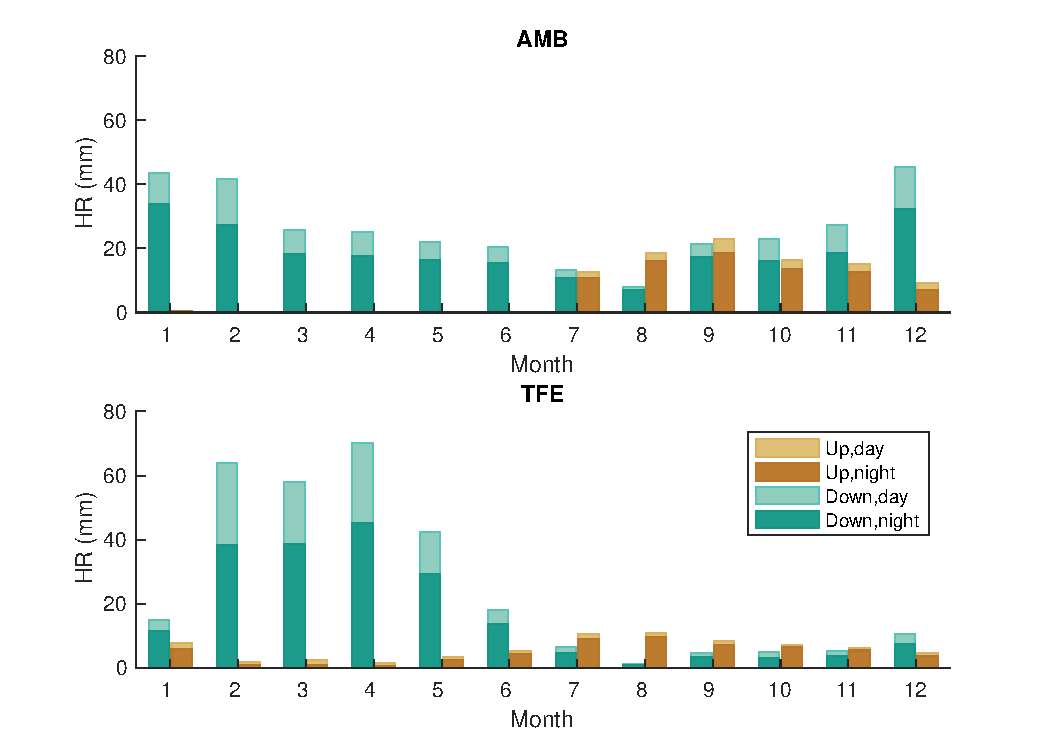
\includegraphics[width=30pc]{../figs2/supphr.pdf}
     \caption{PHS hydraulic distribution during 2003. Alternative version partitioning by direction.}
     \label{supp:hr2}
  \end{figure}
  \clearpage
  
     \clearpage
    \begin{figure}[h]
     \centering
     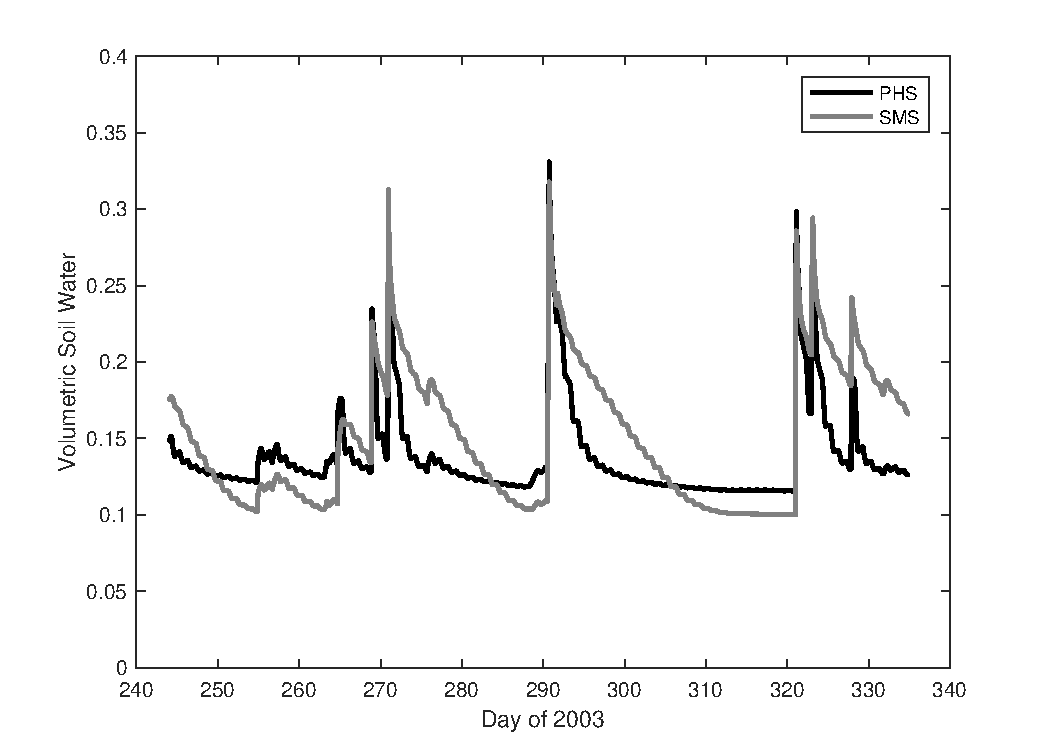
\includegraphics[width=30pc]{../figs2/supplayer2.pdf}
     \caption{Volumetric soil water content in Soil Layer 2 (which spans 2-6cm in depth), for SON-2003, featuring 60\% throughfall exclusion.
     With PHS (black line), the soil layer can dry out much more quickly after rain events.}
     \label{fig9}
  \end{figure}
  
  
        \clearpage
    \begin{figure}[h]
     \centering
     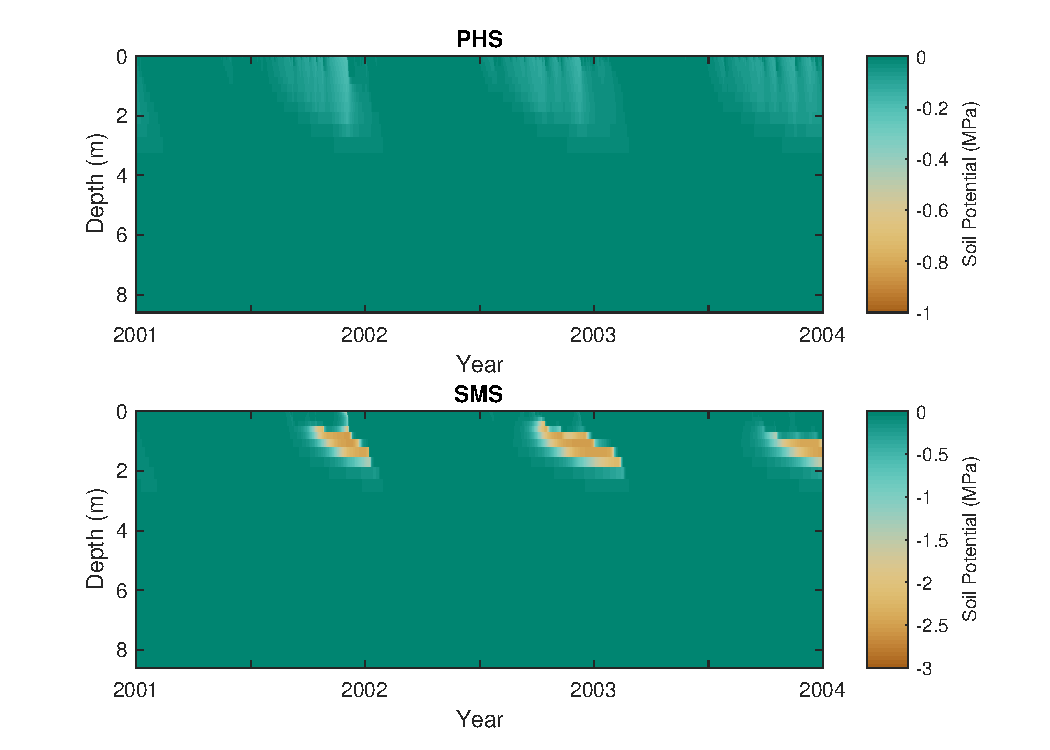
\includegraphics[width=30pc]{../figs2/suppsmp.pdf}
     \caption{Vertical profile of soil water potential (MPa) through time under ambient throughfall conditions, for
     (a) PHS, and 
     (b) SMS.
     Note that color axes are different. }
     \label{supp:smp}
  \end{figure}



\section{Appendix to Model Description}

% Details on water supply
\subsection{Details of Water Supply}

PHS resolves flow across four different segments, soil-to-root, root-to-stem, stem-to-leaf, and leaf-to-transpiration.

Stem-to-leaf. The area bases are sunlit and shaded leaf area, respectively. 
Note that gravity is assumed negligible here. 
Likewise there is no length scaling applied to maximum conductance. 
Therefore the input parameters for $k_{1,\text{max}}$ should be conductances ($s^{-1}$).

\begin{linenomath*} \begin{equation} \begin{aligned}
q_{1a} &= k_{1} \cdot \text{LAI-sun}  \cdot \left( \psi_{\text{stem}}-\psi_{\text{sun-leaf}}\right) \\
q_{1b} &= k_{1} \cdot \text{LAI-shade} \cdot  \left( \psi_{\text{stem}}-\psi_{\text{shade-leaf}}\right)
\end{aligned} \end{equation} \end{linenomath*}

\begin{linenomath*} \begin{equation}
k_{1} = k_{1,\text{max}} \cdot f\left(\psi_{\text{stem}}\right)
\end{equation} \end{linenomath*}

\begin{linenomath*} \begin{equation} \begin{aligned}
f\left(\psi\right)=2^{-\left(\dfrac{\psi}{p_{50}}\right)^{c_k}}
\end{aligned} \end{equation} \end{linenomath*}

Root-to-stem. The area basis is stem area index. 
The parameter is maximum stem xylem conductivity ($K_{2,\text{max}}$).
Stem conductance ($k_2$) is the result of scaling maximum conductivity by the tree height ($h$)
and applying loss relative to maximum conductance via the vulnerability curve $f\left(\psi_{\text{root}}\right)$. 
\begin{linenomath*} \begin{equation}
q_2 = k_2 \cdot  \text{SAI}  \cdot \left( \psi_{\text{root}}-\psi_{\text{stem}}-\rho g h\right)
\end{equation} \end{linenomath*}
\begin{linenomath*} \begin{equation}
k_2 = \dfrac{K_{2,\text{max}}}{h} \cdot f\left(\psi_{\text{root}}\right)
\end{equation} \end{linenomath*}

Soil-to-root. Area basis is RAI in soil layer $i$, which is based on the layer root fraction times the
total root area. Total root area we have as the summed stem and leaf area indices multiplied by a relative
root area parameter ($f_{\text{root}}$).
The vertical root distribution is defined by the layer root fraction ($r_i$), which follows a one-parameter 
(by PFT) power law decay following \citet{jackson1996}.

\begin{linenomath*} \begin{equation}
q_{3,i} = k_{3,i} \cdot  \text{RAI}_i  \cdot \left( \psi_{\text{soil,i}}-\psi_{\text{root}}-\rho g z_i\right)
\end{equation} \end{linenomath*}
\begin{linenomath*} \begin{equation}
\text{RAI}_i=f_{\text{root}} \cdot \left( \text{SAI} + \text{LAI} \right) \cdot r_i
\label{eq:rai}
\end{equation} \end{linenomath*}
\begin{linenomath*} \begin{equation}
k_{3,i} = \dfrac{k_{r,i}+k_{s,i}}{k_{r,i}\cdot k_{s,i}}
\end{equation} \end{linenomath*}
\begin{linenomath*} \begin{equation}
k_{r,i} = \dfrac{K_{r,\text{max}}}{l_i} f \left(\psi_{\text{soil,i}}\right)
\end{equation} \end{linenomath*}
\begin{linenomath*} \begin{equation}
l_i = z_i + x
\end{equation} \end{linenomath*}
\begin{linenomath*} \begin{equation}
k_{s,i} = \dfrac{K_{s,i}}{d}
\end{equation} \end{linenomath*}

The conductance $k_{3,i}$ reflects two resistors in series, from soil-to-root ($k_{s,i}$) and through the
root tissue ($k_{r,i}$).
The root tissue conductance is attenuated via the vulnerability curve framework. 
The input parameter is maximum root xylem conductivity, on the basis of RAI as defined above.
The root conductivity is scaled by the conducting length, which is estimated as the sum of soil layer depth ($z_i$)
and average lateral extent ($x$, static parameter).
The soil conductivity $K_{s,i}$ is calculated from the layer soil matric potential ($\psi_s$) 
and soil properties following \citet{clapp1978} as described in \citet{oleson2013}.
The soil conductance ($k_{s,i}$) is the result of scaling the conductivity by $d$, 
 the distance between roots estimated following \citet{williams1996} and \citet{bonan2014}

The challenge here is obviously getting your head around all the parameters.

% Details on water demand
\subsection{Details of Water Supply}

% Details on phs solution
\subsection{Details of Solution}


The continuity of water flow through the system yields four equations
   \begin{linenomath*} \begin{equation}
   \begin{aligned}
   E_{sun}&=q_{1a}\\
   E_{shade}&=q_{1b}\\
   q_{1a}+q_{1b}&=q_2\\
   q_2&=\sum_{i=1}^{nlevsoi}{q_{3,i}}
   \end{aligned}
   \end{equation} \end{linenomath*}

We seek the set of vegetation water potential values (four unknowns), 

   \begin{linenomath*} \begin{equation}
   \psi=\left[ \begin {array}{c} 
   \psi_{sunleaf}\cr\psi_{shadeleaf}\cr\psi_{stem}\cr\psi_{root}
   \end {array} \right] 
   \end{equation} \end{linenomath*}

that satisfies these equations, as forced by the soil moisture and atmospheric state. 

Each flux on the schematic can be represented in terms of the relevant water potentials. 

Defining the transpiration fluxes:


   \begin{linenomath*} \begin{equation}
   \begin{aligned}
   E_{sun} &= E_{sun,max} \cdot 2^{-\left(\dfrac{\psi_{sunleaf}}{p50_e}\right)^{c_k}} \\
   E_{shade} &= E_{shade,max} \cdot 2^{-\left(\dfrac{\psi_{shadeleaf}}{p50_e}\right)^{c_k}} 
   \end{aligned}
   \end{equation} \end{linenomath*}

Defining the water supply fluxes:

   \begin{linenomath*} \begin{equation}
   \begin{aligned}
   q_{1a}&=k_{1a,max}\cdot 2^{-\left(\dfrac{\psi_{stem}}{p50_1}\right)^{c_k}} \cdot\mbox{LAI}_{sun}\cdot\left(\psi_{stem}-\psi_{sunleaf} \right) \\
   q_{1b}&=k_{1b,max}\cdot 2^{-\left(\dfrac{\psi_{stem}}{p50_1}\right)^{c_k}}\cdot\mbox{LAI}_{shade}\cdot\left(\psi_{stem}-\psi_{shadeleaf} \right) \\
   q_2&=\dfrac{k_{2,max}}{z_2} \cdot 2^{-\left(\dfrac{\psi_{root}}{p50_2}\right)^{c_k}} \cdot SAI \cdot \left( \psi_{root} - \psi_{stem} - \Delta \psi_z  \right) \\
   q_{soil}&=\sum_{i=1}^{nlevsoi}{q_{3,i}}=\sum_{i=1}^{nlevsoi}{k_{3,i}\cdot RAI\cdot\left(\psi_{soil,i}-\psi_{root} + \Delta\psi_{z,i} \right)}
   \end{aligned}
   \end{equation} \end{linenomath*}

We're looking to find the vector $\psi$
that fits with soil and atmospheric forcings while satisfying water flow continuity. 
Due to the model non-linearity, we use a linearized explicit approach, iterating with Newton's method. 
The initial guess is the solution for $\psi$ (vector) from the previous time step. 
The general framework, from iteration $m$ to $m+1$ is:

   \begin{linenomath*} \begin{equation} 
   \begin{aligned}
   q^{m+1}&=q^m+\dfrac{\delta q}{\delta\psi}\Delta\psi \\
   \psi^{m+1}&=\psi^{m}+\Delta\psi
   \end{aligned}
   \end{equation} \end{linenomath*}

So for our first flux balance equation, at iteration $m+1$, we have:

   \begin{linenomath*} \begin{equation} 
   E_{sun}^{m+1}=q_{1a}^{m+1}
   \end{equation} \end{linenomath*}

Which can be linearized to:

   \begin{linenomath*} \begin{equation} 
   E_{sun}^{m}+\dfrac{\delta E_{sun}}{\delta\psi}\Delta\psi=q_{1a}^{m}+\dfrac{\delta q_{1a}}{\delta\psi}\Delta\psi
   \end{equation} \end{linenomath*}

And rearranged to be:

   \begin{linenomath*} \begin{equation} 
   \dfrac{\delta q_{1a}}{\delta\psi}\Delta\psi-\dfrac{\delta E_{sun}}{\delta\psi}\Delta\psi=E_{sun}^{m}-q_{1a}^{m}
   \end{equation} \end{linenomath*}

And for the other 3 flux balance equations:

   \begin{linenomath*} \begin{equation} 
   \begin{aligned}
   \dfrac{\delta q_{1b}}{\delta\psi}\Delta\psi-\dfrac{\delta E_{sha}}{\delta\psi}\Delta\psi&=E_{sha}^{m}-q_{1b}^{m} \\
   \dfrac{\delta q_2}{\delta\psi}\Delta\psi-\dfrac{\delta q_{1a}}{\delta\psi}\Delta\psi-\dfrac{\delta q_{1b}}{\delta\psi}\Delta\psi&=q_{1a}^{m}+q_{1b}^{m}-q_2^{m} \\
   \dfrac{\delta q_{soil}}{\delta\psi}\Delta\psi-\dfrac{\delta q_2}{\delta\psi}\Delta\psi&=q_2^{m}-q_{soil}^{m}
   \end{aligned}
   \end{equation} \end{linenomath*}

Putting all four together in matrix form:

   \begin{linenomath*} \begin{equation} 
   \left[ \begin {array}{c}
   \dfrac{\delta q_{1a}}{\delta\psi}-\dfrac{\delta E_{sun}}{\delta\psi} \cr
   \dfrac{\delta q_{1b}}{\delta\psi}-\dfrac{\delta E_{sha}}{\delta\psi} \cr
   \dfrac{\delta q_2}{\delta\psi}-\dfrac{\delta q_{1a}}{\delta\psi}-\dfrac{\delta q_{1b}}{\delta\psi} \cr
   \dfrac{\delta q_{soil}}{\delta\psi}-\dfrac{\delta q_2}{\delta\psi}
   \end {array} \right]
   \Delta\psi=
   \left[ \begin {array}{c}
   E_{sun}^{m}-q_{1a}^{m} \cr
   E_{sha}^{m}-q_{1b}^{m} \cr
   q_{1a}^{m}+q_{1b}^{m}-q_2^{m} \cr
   q_2^{m}-q_{soil}^{m}
   \end {array} \right]
   \end{equation} \end{linenomath*}

Now to expand the left-hand side, from vector $\psi$ to the four distinct plant water potential nodes, noting that many derivatives are zero (e.g. $\dfrac{\delta E_{sun}}{\delta\psi_{sha}}=0$)

Introducing the notation:
$A\Delta\psi=b$

   \begin{linenomath*} \begin{equation} 
   \Delta\psi=\left[ \begin {array}{c}
   \Delta\psi_{sunleaf} \cr
   \Delta\psi_{shadeleaf} \cr
   \Delta\psi_{stem} \cr
   \Delta\psi_{root}
   \end {array} \right] 
   \end{equation} \end{linenomath*}

   \begin{linenomath*} \begin{equation} 
   A=
   \left[ \begin {array}{cccc}
   \dfrac{\delta q_{1a}}{\delta \psi_{sun}}-\dfrac{\delta E_{sun}}{\delta \psi_{sun}}&0&\dfrac{\delta q_{1a}}{\delta \psi_{stem}}&0\cr
   0&\dfrac{\delta q_{1b}}{\delta \psi_{sha}}-\dfrac{\delta E_{sha}}{\delta \psi_{sha}}&\dfrac{\delta q_{1b}}{\delta \psi_{stem}}&0\cr
   -\dfrac{\delta q_{1a}}{\delta \psi_{sun}}&
   -\dfrac{\delta q_{1b}}{\delta \psi_{sha}}&
   \dfrac{\delta q_2}{\delta \psi_{stem}}-\dfrac{\delta q_{1a}}{\delta \psi_{stem}}-\dfrac{\delta q_{1b}}{\delta \psi_{stem}}&
   \dfrac{\delta q_2}{\delta \psi_{root}}\cr
   0&0&-\dfrac{\delta q_2}{\delta \psi_{stem}}&\dfrac{\delta q_{soil}}{\delta \psi_{root}}-\dfrac{\delta q_2}{\delta \psi_{root}}
   \end {array} \right]
   \end{equation} \end{linenomath*}

   \begin{linenomath*} \begin{equation} 
   b=
   \left[ \begin {array}{c}
   E_{sun}^{m}-q_{b1}^{m} \cr
   E_{sha}^{m}-q_{b2}^{m} \cr
   q_{b1}^{m}+q_{b2}^{m}-q_{stem}^{m} \cr
   q_{stem}^{m}-q_{soil}^{m}
   \end {array} \right]
   \end{equation} \end{linenomath*}

Now we compute all the entries for $A$ and $b$ based on the soil moisture and maximum transpiration forcings and can solve to find:

   \begin{linenomath*} \begin{equation} 
   \Delta\psi=A^{-1}b
   \end{equation} \end{linenomath*}

   \begin{linenomath*} \begin{equation} 
   \psi_{m+1}=\psi_m+\Delta\psi
   \end{equation} \end{linenomath*}

We iterate until $b\to 0$, signifying water flux balance through the system. The result is a final set of water potentials ( $\psi_{root}$, $\psi_{xylem}$, $\psi_{shadeleaf}$, $\psi_{sunleaf}$) satisfying non-divergent water flux through the system. 
The magnitude of the water flux is driven by soil matric potential and unstressed ( $\beta_t=1$) transpiration. 

We use the transpiration solution (corresponding to the final solution for $\psi$) to compute stomatal conductance. The stomatal conductance is then used to compute $\beta_t$. 

   \begin{linenomath*} \begin{equation} 
   \beta_{t,sun} = \dfrac{g_{s,sun}}{g_{s,sun,\beta_t=1}} 
   \end{equation} \end{linenomath*}

   \begin{linenomath*} \begin{equation} 
   \beta_{t,shade} = \dfrac{g_{s,shade}}{g_{s,shade,\beta_t=1}} 
   \end{equation} \end{linenomath*}

The $\beta_t$ values are used in the Photosynthesis module (see section \ref{sect:A}) to apply water stress. 
The solution for $\psi$ is saved as a new variable (vegetation water potential) and is indicative of plant water status.
The soil-to-root fluxes $\left( q_{3,1},q_{3,2},\text{...},q_{3,n}\right)$ are used as the soil transpiration sink in the Richards' equation subsurface flow equations.

\acknowledgments
 = enter acknowledgments here =


%====================
%   REFERENCES
%====================
\nocite{*} 
\bibliography{refs/all}


\listofchanges


\end{document}


